\documentclass[11pt]{article}
\usepackage{ulem}
\usepackage{graphicx}
\usepackage{epstopdf}
\usepackage{amsmath}
\newcommand{\norm}[1]{\left|\left|#1\right|\right|}
\begin{document}
\title{Lesson 1} 
\author{CSPP58001}
\date{\today}
\maketitle

\section{Linear Systems}
The most fundamental aspect of computational science is the solution of
a linear system of equations. At this point we will not worry about why
linear systems arise so frequently and what types of phenomena and processes
they represent. This will be step 2 -- the application of the techniques we learn
to common computational science problems. For now we focus on the definition
and processes for efficiently solving linear system.

We start with the most common and well
defined case -- a {\em square} system of m equations and m unknowns.
This is written generally as:
\begin{eqnarray}
a_{11} x_1 &+& a_{12} x_2 + \ldots + a_{1m}x_m = b_1 \nonumber \\ 
a_{21} x_1 &+& a_{22} x_2 + \ldots + a_{2m}x_m = b_2 \nonumber \\
&\vdots& \nonumber \\ 
a_{m1} x_1 &+& a_{m2} x_2 + \ldots + a_{mm}x_m = b_m \nonumber
\end{eqnarray}
where the $m^2$ $a_{ij}$'s and the m $b$'s are known constants and the goal
is to find  $m x_i$'s that satisfy the equality. For a square system, most typically there will be a single unique
solution to the system. I say "most typically" because as we will see later the
matrix A representing this linear transformation has a small chance of being {\em singular}
(or equivalently of having a zero {\em determinant} and thus being {\em non-invertible} --
all ways of expressing the same concept). In the more typical case where the system
is not singular and a unique solution exists, one of the most common procedures in all of 
computational science is to efficiently find the solution. 

\subsection{Matrix representation}
Linear algebra has developed very concise notation for representing linear systems,
based on {\em matrices} and {\em vectors}. It is likely that most students in cspp58001
have some level of familiarity with these concepts, but this is not required as a basic understanding 
can be attained very easily. I strongly recommend the first few chapters of Strang's {\em Introduction
to Linear Algebra} listed on the course website for a clear and concise review.

In matrix notation we write the linear system above as:
\begin{equation}
Ax=b
\end{equation}
where A is the matrix defined by
\[ \left( \begin{array}{cccc}
a_{11} & a_{12} & \ldots & a_{1m} \\
a_{21} & a_{22} & \ldots & a_{2m} \\
\vdots &  &  &  \\
a_{m1} & a_{m2} & \ldots & a_{mm} \\
 \end{array} \right)\]
$b$ is the {\em column vector} (ie $m \times 1$ matrix) defined by
\[ \left( \begin{array}{c}
b_1 \\
b_2 \\
\vdots \\
b_m
 \end{array} \right)\]
 and $x$ is the column vector of unknowns defined by
\[ \left( \begin{array}{c}
x_1 \\
x_2 \\
\vdots \\
x_m.
 \end{array} \right)\]
 Until the rules of matrix multiplication are defined, matrices just look like collections of numbers indexed by row/column --
 ie we refer, for example to the entry in the third row and fourth column of A as $a_{34}$. There is no point in reproducing
 those rules here -- they are in hundreds of introductory algebra textbooks. The description in Strang is recommended as
 it presents four identical but conceptually unique ways to think about matrix multiplication, each of which has particularly
 advantages later in understanding its role in different operations. We go over these briefly in class. I also strongly recommend
 using Matlab as a way to interactively train yourself to think about matrix operations -- in Matlab these are built in as intrinsic
 operators on matrix and vector types, and the interpreter provides a fun way to test your understanding of the basic operations.
 
 In the system $Ax=b$ above, in this course I will tend to emphasize that A is a matrix and x and b are vectors by using the following
 notation:
 \begin{equation}
% \uuline{A} \uline x = \uline b
\underline{\underline{A}} \underline{x} = \underline{b}
 \end{equation}
 -- ie each underline represents one dimension. Scalar values are thus not underlined. Once you gain more familiarity with linear
 algebra notation this extra syntax should no longer be necessary as the type can typically be recognized by context.
 
 \subsection{Simple example}
 It's useful to go through a simple example to make the above more concrete. Consider the following linear system:
  \\
\begin{eqnarray}
2x_1 + x_2 &=& 4 \\ 
x_1 - x_2 &=& -1 \nonumber
 \end{eqnarray}
It should be clear that the vector $x = [1\; 2]^T$ solves this equation, where we use the $[]^T$ symbol to denote the transpose -- ie
switching of rows/columns so that $x$ is ca column vector (it is easier to write as a row vector in text).

There are two conceptually distinct but ultimately identical ways to view the solution to this system. The most common way is to consider
the rows. In two dimensions we can easily graph the line representing each equation (row). The solution is then their intersection.
\begin{figure}[h!]
 \begin{center}
 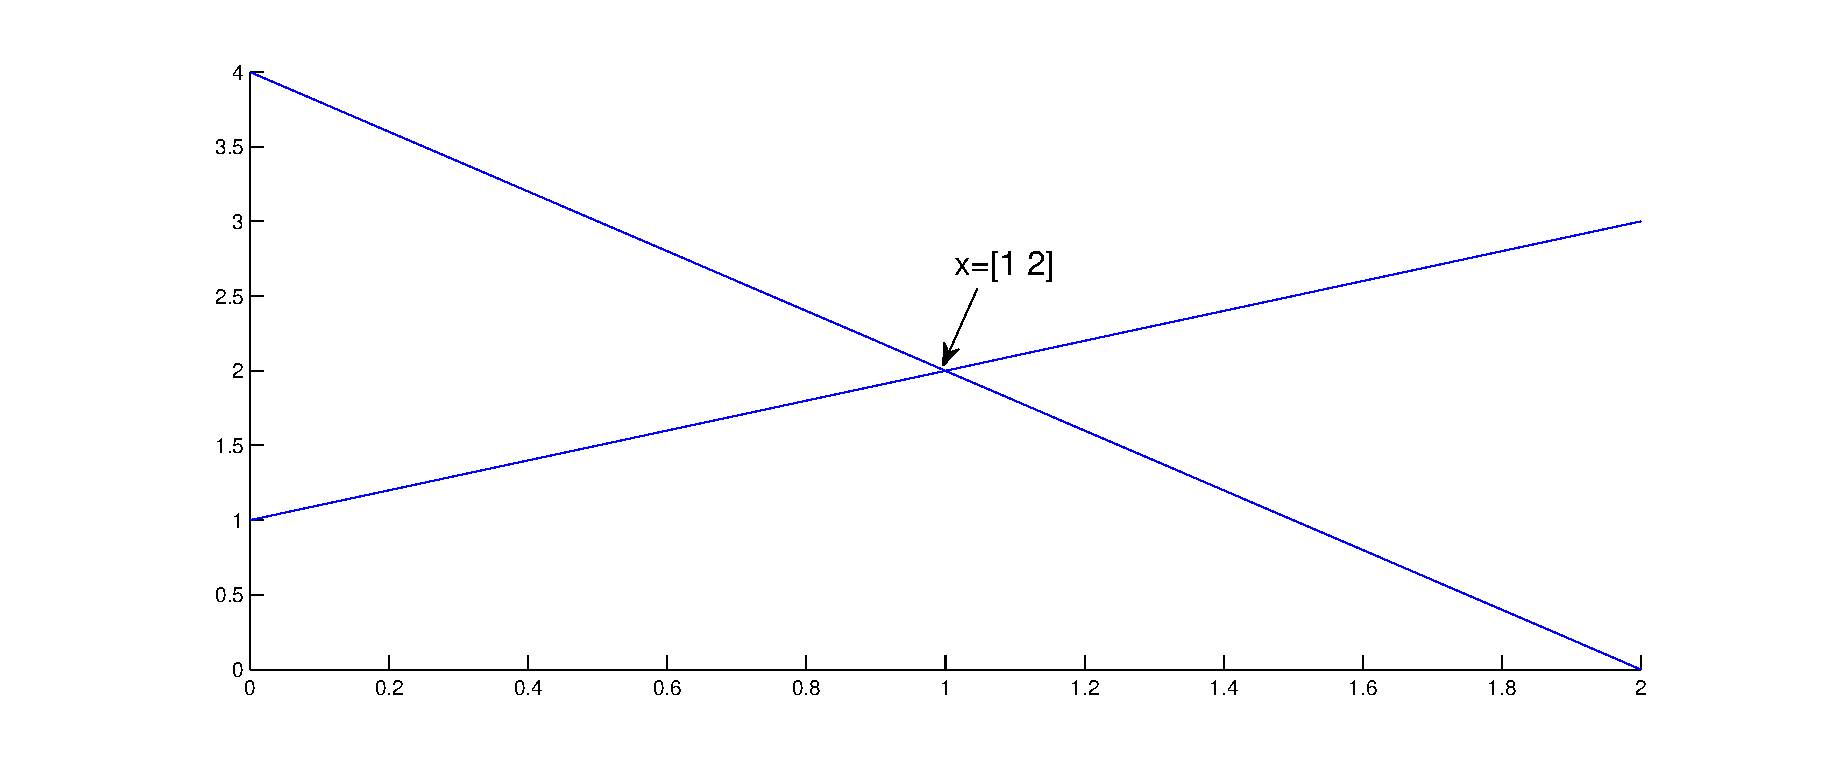
\includegraphics[width=3.5in]{fig1.eps}
\end{center}
\caption{\small {\it Solution to the example linear system can be viewed as the intersection of the row equations}}.
\label{fig:comm-time}
\end{figure}
Looking at it this way it is also clear what can go wrong. If the two equations are parallel -- ie if one equation is simply a multiple of the other -- then there is clearly no solution (as we will
see this would result in a singular matrix). Also, if the lines are identical then there are infinitely many solutions. While it is hard to extend this reasoning geometrically beyond three dimensions,
the same properties and definitions hold and it is useful to conceive of it in terms of the lower dimensional case.

The second way of looking at this same process is to consider matrix multiplication by columns. It should be easy to see that matrix multiplication can also
be expressed as:
\[
x_1 
\begin{bmatrix}
2 \\
1
\end{bmatrix}
+
x_2
\begin{bmatrix}
1 \\
-1
\end{bmatrix}
= 
\begin{bmatrix}
4 \\
-1
\end{bmatrix}\]
ie the solution is given as the correct linear combination of the column vectors. Viewed this way together with the graphical rules of vector addition (head to tail), we can then think
of the solution as the exact combination of the sum of the first column and the second column such that they exactly sum to the solution. I leave it as a simple exercise to graph this
by hand or in matlab and convince yourself that you obtain the correct answer. Viewed this way we can begin to see concepts that will become important later in the course -- the
idea of vectors that {\it span} a space, a {\it basis}, orthogonality, and again linear independence. For now it is important to keep the column view in mind as well as the row view.

\section{Automating the process -- Guassian elimination}
When the dimension of the linear system is small the solution can be obtained graphically or in an {\it ad hoc} manner (e.g. by inspection or trial and error). When the system
becomes large this is no longer feasible, and we seek a reproducible algorithm that will hopefully reliably provide the correct answer. The most fundamental and canonical
of all such algorithms is {\it Gaussian elimination}(GE), and thus it will provide our starting point for computational linear solvers. Even when GE isn't competitive with more 
sophisticated algorithms, the basic ideas and operations often either underlie or form an important part of the more advanced algorithm. Often, GE is adequate in and of itself.

The basic idea of elimination is to write the a's and b's as a single augmented matrix (the x's are implied but do not need to appear explicitly) and consider the set of operations
that can legally be performed on this matrix without changing the solution. Such an approach is easy to translate into a computer algorithm because it simply involves manipulation
of an array of numbers.

There are three critical operations that we can perform on our augmented matrix without altering the solution:
\begin{enumerate}
\item Multiply any row by a constant
\item Replace any row by a linear combination of other rows
\item Swap any two rows
\end{enumerate}
Note that we need to look more deeply into these operations when considering floating point representation on a computer (accumulated roundoff error become an issue).
However, if we consider initially the ideal case of perfect precision, all of these operations should preserve exactly the solution.

The goal is to use the three operations above to reduce the system to an equivalent {\it upper triangular} system. Again, by equivalent I mean to say "with the same solution".
An upper triangular matrix is simply one whose values are all zero beneath the main diagonal, for example for a $3\times3$ matrix:
\[
U= \begin{bmatrix} 
a_{11} & a_{12}  & a_{13} \\
0 & a_{21} & a_{22}\\
0 & 0 & a_{33}
\end{bmatrix}
\]
Once the system has been transformed to an upper triangular matrix, we will see that the solution is easy to obtain using {\it backsubstitution}.

\subsection{example}
To demonstrate GE it is useful to start with a slightly larger system -- we'll use:
\[
A = 
\begin{bmatrix}
1 & 4 & 3 & -11 \\
6 & 9 & 8 & -9 \\
-5 & 6 & 3 & 13 \\
8 & 3 & -7 & 6 
\end{bmatrix},
b = 
\begin{bmatrix}
41 \\ 31 \\ 2 \\ -31
\end{bmatrix}
\]
where the problem is rigged to give an integer solution (don't expect this in general).

The elimination algorithm then simply loops over columns of the augmented matrix, and for each column it
changes the value of the entry just below the diagonal (the diagonal is called the {\it pivot} in a square matrix)
to zero, transforming the matrix to upper diagonal. To accomplish this while preserving the solution, we simply
subtract the correct multiple of the pivot row from the row that contains the value that we wish to change to zero.
We begin by writing the augmented matrix:
\[
A | b = 
\begin{bmatrix}
1 & 4 & 3 & -11 & 41 \\
6 & 9 & 8 & -9 & 31\\
-5 & 6 & 3 & 13 & 2\\
8 & 3 & -7 & 6 & -31 
\end{bmatrix},
\]
%%%%%%%%%%%%
{\it step 1}: Start at column 1. Identify the pivot ($a_{11} = 1$). Subtract 6 times row 1 from row 2
and replace row 2 with the result:
\[
\begin{bmatrix}
1 & 4 & 3 & -11 & 41 \\
0 & 15 & 10 & -57 & 213\\
-5 & 6 & 3 & 13 & 2\\
8 & 3 & -7 & 6 & -31 
\end{bmatrix},
\]
{\it step 2}: Add 4 times row 1 to row 3 and replace row 3 with the result:
\[
\begin{bmatrix}
1 & 4 & 3 & -11 & 41 \\
0 & 15 & 10 & -57 & 213\\
0 & 26 & 18 & -42 & 206\\
8 & 3 & -7 & 6 & -31 
\end{bmatrix},
\]
%%%%%%%%%%%%
{\it step 3}: Subtract 8 times row 1 with row 4 and replace row 4 with the result:
\[
\begin{bmatrix}
1 & 4 & 3 & -11 & 41 \\
0 & 15 & 10 & -57 & 213\\
0 & 26 & 18 & -42 & 206\\
0 & 29 & 31 & -94 & 359
\end{bmatrix},
\]
Simply repeat this process for columns 2, 3, and 4, zeroing out only those
values beneath the diagonal. In column 2, for example, the pivot value would
be $a_{22} = 15$. The resulting upper triangular matrix should be:
\[
\begin{bmatrix}
1 & 4 & 3 & -11 & 42 \\
0 & -15 & -10 & 57 & -221\\
0 & 0 & .667 & 56.8 & -171.1\\
0 & 0 & 0 & 977.8 & -2933.4
\end{bmatrix},
\]


Once the upper triangular matrix is formed, the final step in determining the solution is referred to as {\it backsubstitution}. 
We simply start at the bottom and build the elements of $x$ in reverse order.
%%%%%%%%
Step 1: solve for $x_4$ using the last equation:
$$977.8x_4 = 2933.4$$ or $$x_4 = -3.0$$
%%%%%%%%%%%
Step 2: solve for $x_3$ using the third (next to last) equation:
$$.667 x_3 + 56.8 (-3.0)= -171.1$$
This can be solved easily in terms of $x_3$ as $$x_3 = -1.0$$
This process then continues until the final solution is obtained.
The basic iteration is:
\begin{equation}
x_i = \frac{1}{a'_{ii}}\left[ b'_i - \sum_{j=i+1}^N a'_{ij}x_j\right].
\end{equation}

An import very basic exercise is to code GE in your favorite language
as well as in Matlab, whose semantics allow a very concise representation
of algorithms that can be express in terms of matrix operations. Since there
are hundreds of examples on the web and in dozens of textbooks, we
do this as a group in-class coding exercise. We note the ways in which
our code differs from, e.g., the example code in Numerical Recipes.

Another important question to ask is how the GE set of operations can
be represented themselves as linear transformations (ie matrix operations).
This is a good exercise in matrix manipulations and appears on homework 1.

\subsection{what can go wrong}
The basic GE algorithm has some potential failure modes. The most
obvious occurs when the value of a pivot happens to be zero. For example,
if the matrix A above were instead:
\[
A = 
\begin{bmatrix}
1 & 4 & 3 & -11 \\
6 & 0 & 8 & -9 \\
-5 & 6 & 3 & 13 \\
8 & 3 & -7 & 6 
\end{bmatrix},
\]
In this case we clearly cannot use $A_{22}$ as a pivot element to eliminate the entries beneath
it. Instead we simply check for a zero pivot and, if one is detected, the algorithm swaps with a row beneath
beneath that has a non-zero pivot. Which row is best? It turns out that to minimize roundoff error we 
typically select the row with the largest pivot value (actually, even when the pivot isn't zero we often
do this to minimize roundoff error). What if no non-zero pivots exist? If this occurs, there is no unique
solution to the system -- as we mentioned earlier, A is singular.

Other issues involve the accumulation of error due to roundoff in decimal representation. To understand
these more deeply we have to dig into floating point representation in a little bit of depth. This will be
covered in lecture 2. 

\section{Matrix inverse}
Though it is not competitive performance wise with GE, a similar algorithm called Gauss-Jordan can provide
both the solution and the inverse matrix $A^{-1}$, where the inverse of a square matrix is defined such that
$$A A^{-1} = A^{-1} A = I$$ where I is the {\it identity matrix}, ie in the case of a $3\times3$ matrix
\[
I = 
\begin{bmatrix}
1 & 0 & 0 \\ 0 & 1 & 0 \\ 0 & 0 & 1
\end{bmatrix}
\]
The inverse of a matrix acts very much like the reciprocal of a scalar. Analogous to the scalar value 0, if a matrix
is singular then its inverse does not exist. We mention briefly that the {\it determinant} gives a quick test
of the invertibility of a matrix -- specifically, if the determinant is not equal to zero, the matrix is guaranteed
to be invertible. Matlab contains the {\it} operator that acts on matrices to compute the determinant.
We briefly mention determinant algorithms when we study eigenvalues later in the course.

The so-called Guass-Jordan (GJ) algorithm is an easy way to compute both the solution to a matrix and its inverse.
There are better ways, so in some sense GJ in only of pedagogical interest. Still, it can be useful and provides a good
conceptual basis for understanding a number of related topics.

To carry out CJ, we perform the same basic steps as GE, with two additions:
\begin{enumerate}
\item eliminate all entries both above and below the diagonal.
\item scale the diagonal entries to a value of 1.
\end{enumerate}

ex. 
\[
[A | b] = 
\begin{bmatrix}
1 & 1 & 2 & 9 \\
2 & 4 & -3 & 1 \\
3 & 6 & -5 & 0 \\
\end{bmatrix},
\]
%%%
By following the elimination process for all non-diagonal entries and scale the diagonal to 1, we get
\[
\begin{bmatrix}
1 & 0 & 0 & 1 \\
0 & 1 & 0 & 2 \\
0 & 0 & 1 & 3 \\
\end{bmatrix},
\]
%%%%%%
It should be clear that the solution can be read directly from the rightmost column. Furthermore, if we
carry out the exact same row operations on the identity matrix $I$, by definition we will have the inverse --
since the transformation that turned the original A into $I$ is by definition $A^{-1}$, then applying
this same set of operations to $I$ is equivalent to $A^{-1} I = A^{-1}$. Test this by performing row operations
on the identity matrix and verifying that the result, when multiplied by $b$, gives the solution to the system.
Note that in general this is not a great idea when we begin to consider the errors introduced by floating point.
Some useful matlab commands relevant to this are {\it inv(A)} to compute a matrix inverse, and {\it rref(A)}
to compute the {\it reduced row echelon form} of $A$, which for the augmented square matrix amounts
to the process described above.

\end{document}
